\documentclass{article}
\usepackage{tikz}
\usetikzlibrary{arrows.meta, calc, positioning}

\begin{document}

\section*{SIMPLE MAIN MODEL}

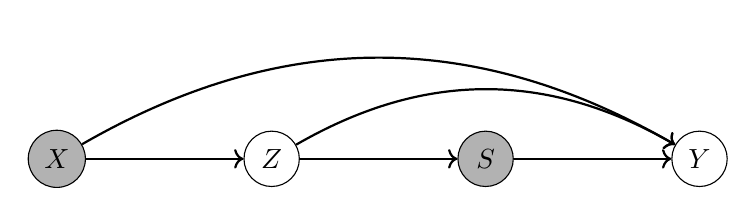
\begin{tikzpicture}[->,
    node distance=2cm,
    main/.style={circle, draw, fill=black!30, minimum size=20pt},
    latent/.style={circle, draw, minimum size=20pt},
    arrow/.style={thick}]
    
    \node[main]  (x) {$X$};
    \node[latent, right=of x] (z) {$Z$};
    \node[main, right=of z]    (s) {$S$};
    \node[latent, right=of s] (y) {$Y$};
    
    \path[arrow]
    (x) edge (z)
        edge[bend left] (y)
    
    (z) edge (s)
        edge[bend left] (y)
    
    (s) edge (y);
    
\end{tikzpicture}

\section*{GENERAL MAIN MODEL}

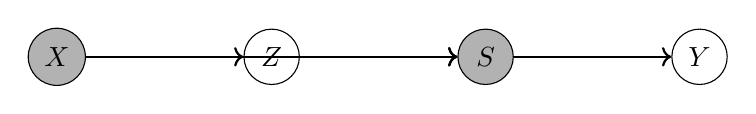
\begin{tikzpicture}[->,
    node distance=2cm,
    main/.style={circle, draw, fill=black!30, minimum size=20pt},
    latent/.style={circle, draw, minimum size=20pt},
    arrow/.style={thick}]
    
    \node[main]  (x) {$X$};
    \node[latent, right=of x] (z) {$Z$};
    \node[main, right=of z]    (s) {$S$};
    \node[latent, right=of s] (y) {$Y$};
    
    \path[arrow]
    (x) edge (z)
    
    (z) edge (s)
    
    (x) edge (s)
    
    (s) edge (y);
    
\end{tikzpicture}

\end{document}